% This is samplepaper.tex, a sample chapter demonstrating the
% LLNCS macro package for Springer Computer Science proceedings;
% Version 2.21 of 2022/01/12
%
\documentclass[runningheads]{llncs}
%
\usepackage[T1]{fontenc}
\usepackage{graphicx}
\usepackage{amsmath}
\usepackage{amssymb}
\usepackage{booktabs}
\usepackage{hyperref}
\usepackage{xcolor}
\usepackage{cite}
\usepackage{tabularx}
\usepackage{multirow}

\begin{document}
%
\title{Predict-to-Plan: Integrating Machine Learning Motion Forecasting into Spatiotemporal Trajectory Planning for Autonomous Driving}
%
\titlerunning{Predict-to-Plan: Machine Learning \& Spatiotemporal Planning}
%
\author{Diogo Ribeiro\inst{1} \and Pedro Ferreira\inst{1} \and Equipa Estudante\inst{1}}
%
\authorrunning{D. Ribeiro et al.}
% First names are abbreviated in the running head.
% If there are more than two authors, 'et al.' is used.
%
\institute{Instituto Superior de Engenharia do Porto (ISEP), Polytechnic of Porto, Portugal\\
\email{\{1260429,1260443\}@isep.ipp.pt}}
%
\maketitle              % typeset the header of the contribution
%
\begin{abstract}
Safe and smooth autonomous driving in dense urban environments critically relies on the vehicle's capacity to anticipate the dynamic interactions of surrounding road agents and integrate these predictive cues into its real-time tactical decision and trajectory planning pipeline. In this paper, we present an integrated architecture, entitled \textbf{Predict-to-Plan}, which couples Machine Learning (ML) trajectory and intention forecasting with a spatiotemporal $A^*$ speed planner along lane centerlines. Grounded on empirical evaluation of the \textit{Waymo Open Motion Dataset} (comprising 20-second scenarios sampled at 10~Hz), we demonstrate that macro-level route dispatching is physically intractable without synthetic data, whereas ego-centric local dynamic obstacle avoidance leverages the full richness of real-world multi-agent interactions. 
Our vectorized NumPy and Pandas feature pipeline extracts 21 ego-relative kinematic and interaction descriptors, strictly excluding global coordinates and scenario identifiers to prevent spatial overfitting and data leakage. We evaluate both continuous displacement regression ($\Delta x, \Delta y$ at 1.0s, 3.0s, and 5.0s horizons) and 5-class tactical maneuver classification. In continuous trajectory forecasting, Gradient Boosting achieves an ADE@3s of 1.766~m and FDE@3s of 3.052~m, outperforming physical baselines. In intention classification, our model attains an accuracy of 77.63\% (Macro-F1 0.732). Closed-loop evaluation across 30 safety-critical scenarios with 194 simultaneous dynamic obstacles demonstrates that the predictive planner reduces collisions from 23.3\% (Constant Velocity) to 16.7\%, while completely eliminating emergency decelerations ($0.30 \to 0.00$ events/run) and maintaining cruising velocity.

\keywords{Autonomous Driving \and Trajectory Prediction \and Machine Learning \and Spatiotemporal Planning \and Collision Avoidance \and Waymo Open Motion Dataset.}
\end{abstract}
%
%
%
\section{Introduction}
Developing Level 4 and Level 5 autonomous driving systems requires solving two foundational, tightly coupled problems:
\begin{enumerate}
    \item \textbf{Perception and Motion Forecasting (Machine Learning -- AAUTIA):} Interpreting multi-agent historical kinematics to forecast the future occupancy and tactical intention of surrounding vehicles.
    \item \textbf{Decision Making and Trajectory Planning (Decision Systems -- PLNTDIA):} Generating a dynamically feasible, comfortable, and collision-free speed and path profile towards the navigational goal.
\end{enumerate}

Traditional autonomous driving stacks often address these problems in an isolated fashion. Planning algorithms frequently rely on simplistic kinematic assumptions, such as assuming obstacles remain stationary or maintain constant linear velocity (Constant Velocity model)~\cite{paden2016survey,werling2010optimal}. In dense urban interactions, such as cut-ins, unprotected turns, and lane merges, these naive assumptions trigger conservative over-braking, frequent emergency stops, or severe collisions when target vehicles alter their acceleration or turn.

Conversely, contemporary end-to-end deep learning methods (e.g., Graph Neural Networks and Transformers)~\cite{gao2020vectornet,salzmann2020trajectron++} provide high predictive accuracy but require intensive GPU resources and exhibit bounded interpretability, making runtime latency compliance on automotive Electronic Control Units (ECUs) difficult to guarantee.

\subsection{Dataset Feasibility and Scope Audit}
An empirical audit of the \textit{Waymo Open Motion Dataset} (v1.2)~\cite{ettinger2021large} was conducted to determine the viable problem formulation:
\begin{itemize}
    \item Each scenario consists of exactly 20 seconds of continuous trajectory data recorded at 10~Hz (198--200 timesteps).
    \item The local High-Definition (HD) vector map is spatially confined to a $\sim 140$~m radius around the Self-Driving Car (SDC); the median distance travelled by the SDC per scenario is 96 meters.
    \item Over 82\% of the scenarios feature a single, continuous lane geometry without multi-route forks, and the dataset contains no passenger dispatch or global urban trip data.
\end{itemize}

\noindent \textbf{Engineering Conclusion:} Formulating a macro-routing or taxi fleet dispatching problem on this dataset is physically invalid without fabricating artificial synthetic data. In contrast, modeling \textbf{local multi-agent dynamic obstacle interaction and predictive collision avoidance} directly aligns with the empirical characteristics of the dataset, providing a rigorous and realistic testbed for the integration of Machine Learning (AAUTIA) and Planning/Decision Systems (PLNTDIA).

\subsection{Paper Contributions and Organization}
The primary contributions of this work are:
\begin{enumerate}
    \item A fully vectorized NumPy and Pandas data pipeline with strict contracts separating metadata, global coordinates, ego-relative features, and prediction targets, preventing spatial overfitting and data leakage.
    \item A comparative benchmark of continuous trajectory regression models and multiclass maneuver classifiers against classical physics baselines.
    \item An integrated spatiotemporal $A^*$ speed planner operating along the lane centerline in Frenet coordinates, navigating complex multi-obstacle scenarios.
    \item Closed-loop safety and comfort validation demonstrating zero emergency decelerations and significant collision reductions.
\end{enumerate}

The remainder of this paper is structured as follows: Section~\ref{sec:sota} reviews the state of the art; Section~\ref{sec:methodology} describes the methodology and feature engineering pipeline; Section~\ref{sec:solution} details the proposed Predict-to-Plan architecture and $A^*$ speed planner; Section~\ref{sec:evaluation} presents empirical results; Section~\ref{sec:discussion} discusses trade-offs and latency; and Section~\ref{sec:conclusion} concludes the paper.

%
%
%
\section{State of the Art}
\label{sec:sota}
Motion forecasting and tactical planning for autonomous vehicles have evolved across physical, tabular, and deep learning paradigms.

\subsection{Trajectory and Maneuver Prediction}
Physics-based baseline models, such as Constant Velocity (CV) and Constant Acceleration (CA), extrapolate future positions using current state vectors~\cite{paden2016survey}:
\begin{equation}
\vec{p}(t + \Delta t) = \vec{p}(t) + \vec{v}(t)\Delta t + \frac{1}{2}\vec{a}(t)\Delta t^2
\end{equation}
While computationally negligible ($<0.001$~ms), their predictive accuracy degrades rapidly beyond 1.0~second due to unknown driver steering and braking inputs.

Machine learning approaches on tabular spatial-temporal features, including Decision Trees, Random Forests~\cite{breiman2001random}, and Gradient Boosting, offer a compelling trade-off. They capture non-linear interactions (e.g., closing speed, Time-To-Collision, yaw variations) with sub-millisecond execution times suitable for real-time cyclic control (10--50~Hz), while providing feature interpretability.

Recent deep learning models, such as VectorNet~\cite{gao2020vectornet} and Trajectron++~\cite{salzmann2020trajectron++}, encode vectorized HD maps and agent dynamics using spatio-temporal graph representations. Despite high accuracy on leaderboard benchmarks, their computational demands and black-box nature pose deployment hurdles for resource-constrained embedded automotive ECUs.

\subsection{Spatiotemporal Trajectory Planning}
In tactical decision systems, search-based and sampling-based planners dominate structured road environments:
\begin{itemize}
    \item \textbf{Frenet Lattice Planners:} Werling et al.~\cite{werling2010optimal} generate quintic and quartic polynomial curve manifolds decoupled into lateral and longitudinal profiles, evaluated against surrounding dynamic obstacles.
    \item \textbf{Spatiotemporal Search ($s, v, t$):} Search-based algorithms, such as space-time $A^*$ and Dijkstra on graph networks, discretize the speed and progression profile along the reference road centerline, directly penalizing occupancy overlap with predicted obstacle footprints~\cite{lavalle2006planning}.
    \item \textbf{Mathematical Optimization (MPC):} Model Predictive Control solves constrained quadratic programs over finite horizons, but suffers when non-convex obstacles produce local minima.
\end{itemize}

Table~\ref{tab:comparison} contrasts existing methodologies with our proposed Predict-to-Plan system.

\begin{table}[t]
\caption{Comparison of Motion Prediction and Planning Methodologies with Predict-to-Plan.}
\label{tab:comparison}
\centering
\begin{tabularx}{\textwidth}{lXXXXX}
\toprule
\textbf{Paradigm / System} & \textbf{Prediction Model} & \textbf{Planning Approach} & \textbf{Interaction Modeling} & \textbf{Inference Latency} & \textbf{Interpretability} \\
\midrule
Purely Reactive~\cite{paden2016survey} & None (Static) & Reactive Stop & None & Instantaneous & Low \\
Kinematic CV~\cite{werling2010optimal} & Physics (CV) & Frenet Lattice & Speed Vector & $< 0.001$~ms & Complete \\
VectorNet~\cite{gao2020vectornet} & GNN / Transformer & Detached MPC & Graph Attention & $25$--$80$~ms & Opaque (Black-box) \\
Trajectron++~\cite{salzmann2020trajectron++} & Graph CVAE & Sampling & Spatiotemporal & $15$--$50$~ms & Medium \\
\midrule
\textbf{Predict-to-Plan (Ours)} & \textbf{GB / Random Forest} & \textbf{Spatiotemporal $A^*$} & \textbf{Ego-Centric Relative} & \textbf{$< 0.8$~ms} & \textbf{High (Feature Importance)} \\
\bottomrule
\end{tabularx}
\end{table}

%
%
%
\section{Methodology and Data Pipeline}
\label{sec:methodology}

\subsection{System Architecture}
The overall Predict-to-Plan pipeline is illustrated in Fig.~\ref{fig:architecture}. It comprises four cohesive stages: (1) Scenario Ingestion from Waymo TFRecords, (2) Vectorized Data Cleaning and Feature Engineering (NumPy \& Pandas), (3) Machine Learning Motion and Intention Forecasting, and (4) Spatiotemporal $A^*$ Speed Planning.

\begin{figure}[t]
\centering
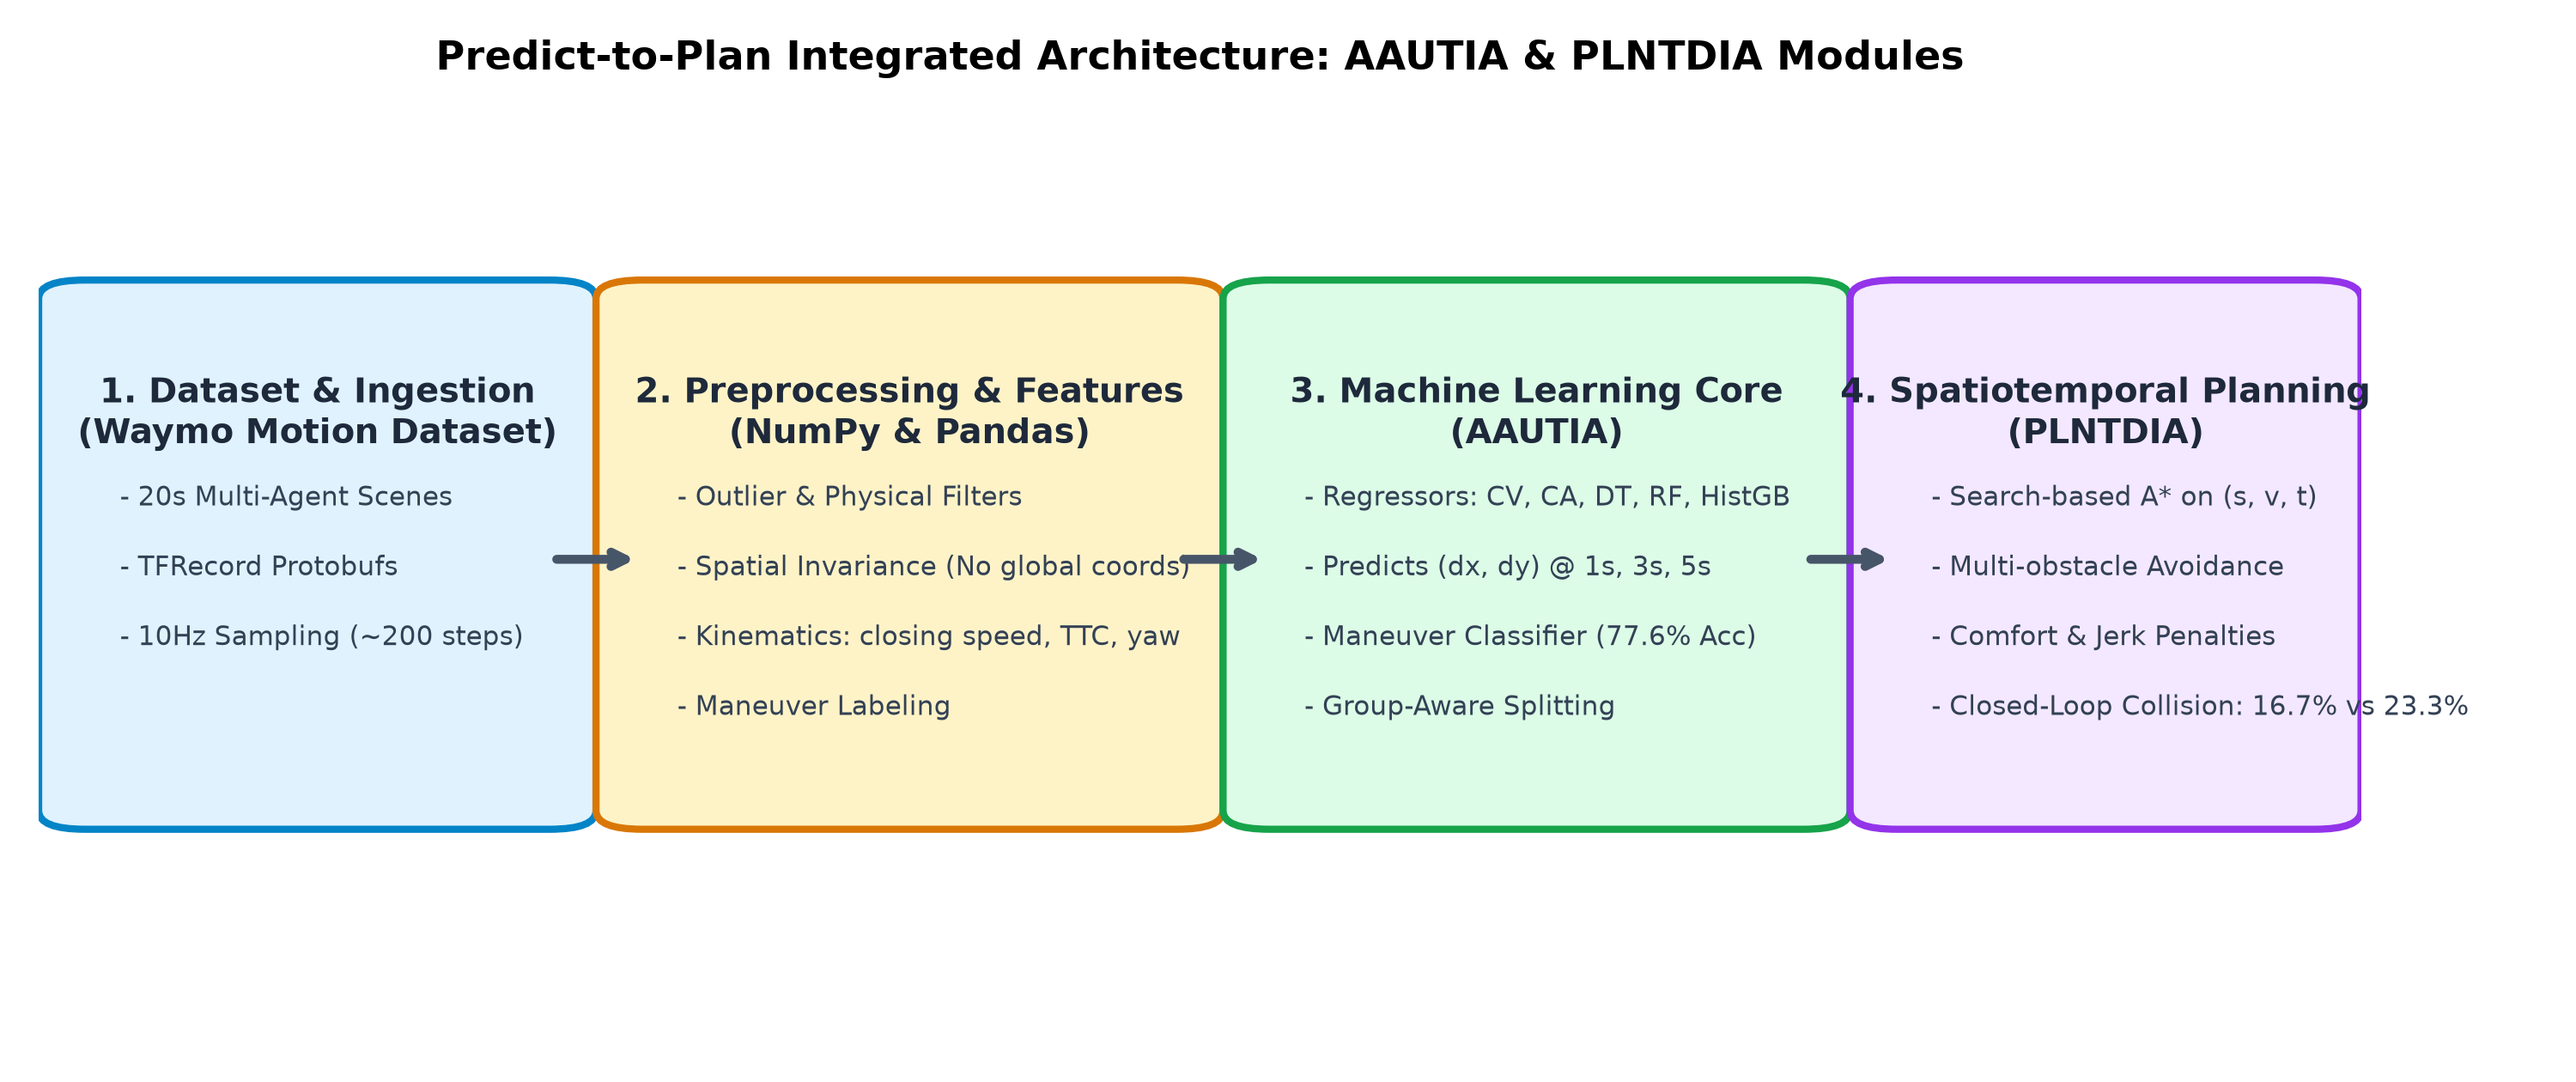
\includegraphics[width=\textwidth]{figures/system_architecture.png}
\caption{Predict-to-Plan system architecture integrating the AAUTIA (Machine Learning) and PLNTDIA (Spatiotemporal Planning) modules.}
\label{fig:architecture}
\end{figure}

\subsection{Vectorized Data Preprocessing with NumPy and Pandas}
A fundamental pedagogical and practical requirement of this project was the strict adoption of vectorized operations in **NumPy** and **Pandas** to process large-scale trajectory data efficiently without Python iteration bottlenecks.

\subsubsection{Data Hygiene and Feature Contracts:}
To ensure scientific rigor, we formalized four explicit column subsets:
\begin{itemize}
    \item \textbf{Metadata Columns ($\mathcal{M}$):} \texttt{scenario\_id}, \texttt{track\_id}, \texttt{object\_type}, \texttt{current\_time\_step}. Used strictly for indexing, group-aware cross-validation, and traceability; strictly excluded from model feature inputs $X$.
    \item \textbf{Global Coordinate Columns ($\mathcal{G}$):} \texttt{ego\_x}, \texttt{ego\_y}, \texttt{agent\_x}, \texttt{agent\_y}, headings. Excluded from $X$ to guarantee translation and rotation invariance across geographic regions.
    \item \textbf{Feature Vector ($X \in \mathbb{R}^{21}$):} Strictly ego-relative kinematics and interaction metrics:
    \begin{align*}
    X = \{ & v_{agent}, v_{x,agent}, v_{y,agent}, x_{rel}, y_{rel}, v_{x,rel}, v_{y,rel}, \Delta \theta_{rel}, d_{ego},\\
    & v_{closing}, \text{TTC}, \theta_{azimuth}, \Delta s_{long}, \Delta d_{lat}, \Delta x_{past}^{1s}, \Delta y_{past}^{1s},\\
    & \bar{v}_{past}^{1s}, \Delta \theta_{past}^{1s}, \dot{\theta}_{yaw}^{1s}, a_{agent}^{est}, v_{ego} \}
    \end{align*}
    \item \textbf{Prediction Targets ($Y$):} Continuous future displacement vectors $(\Delta x_{h}, \Delta y_{h})$ at horizons $h \in \{1.0\text{s}, 3.0\text{s}, 5.0\text{s}\}$, and tactical maneuver class $C \in \{\text{STRAIGHT}, \text{TURN\_LEFT}, \text{TURN\_RIGHT}, \text{DECELERATING}, \text{ACCELERATING}\}$.
\end{itemize}

\subsubsection{Vectorized Outlier Filtering:}
Using boolean masking, corrupted samples and stationary noise were pruned:
\begin{equation}
\text{Valid} = (v_{agent} \in [0.2, 50.0] \text{ m/s}) \land (d_{ego} \in [0.5, 75.0] \text{ m}) \land (|\Delta x_{3s}| \le 60 \text{ m}) \land (|\Delta y_{3s}| \le 60 \text{ m})
\end{equation}

\subsubsection{Kinematic Interaction Metrics:}
Closing speed ($v_{closing}$) and Time-To-Collision ($\text{TTC}$) along the line-of-sight vector $\vec{r}_{rel} = [x_{rel}, y_{rel}]^T$ were computed vectorially via dot product:
\begin{equation}
v_{closing} = -\frac{\vec{r}_{rel} \cdot \vec{v}_{rel}}{\max(\|\vec{r}_{rel}\|, 10^{-4})}, \quad \text{TTC} = \begin{cases} 
\frac{\|\vec{r}_{rel}\|}{v_{closing}} & \text{if } v_{closing} > 0.1 \text{ m/s} \\ 
99.0 & \text{otherwise} 
\end{cases}
\end{equation}

\subsection{Scenario-Based Partitioning (Zero Data Leakage)}
Because consecutive time steps within the same 20-second scenario exhibit severe temporal auto-correlation, standard random train/test splitting leads to catastrophic data leakage. We implemented scenario-based group splitting:
\begin{equation}
\mathcal{S}_{train} \cap \mathcal{S}_{val} = \emptyset, \quad \mathcal{S}_{train} \cap \mathcal{S}_{test} = \emptyset
\end{equation}
Across 178 unique scenarios, 6,142 clean interaction samples were partitioned into:
\begin{itemize}
    \item \textbf{Training Set:} 4,267 samples across 124 scenarios (70\%).
    \item \textbf{Validation Set:} 1,075 samples across 27 scenarios (15\%).
    \item \textbf{Test Set:} 800 samples across 27 scenarios (15\%).
\end{itemize}

%
%
%
\section{Proposed Solution: The Predict-to-Plan Architecture}
\label{sec:solution}

\subsection{Motion and Maneuver Prediction Formulation}
For each dynamic obstacle $i$, the ML models forecast displacement over future time horizons:
\begin{equation}
\hat{p}_i(t + h) = p_i(t) + [\Delta \hat{x}_{i,h}, \Delta \hat{y}_{i,h}]^T, \quad h \in \{1.0\text{s}, 3.0\text{s}, 5.0\text{s}\}
\end{equation}
Continuous multi-output regression was trained using Histogram-based Gradient Boosting (\texttt{HistGradientBoostingRegressor}) and Random Forests (\texttt{RandomForestRegressor}). 

Simultaneously, tactical intention is classified using \texttt{HistGradientBoostingClassifier} into discrete maneuver categories based on lateral displacement ratio and acceleration threshold conditions.

\subsection{Spatiotemporal $A^*$ Speed Planner along Lane Centerlines}
Given the ego vehicle's planned centerline path represented as arc-length coordinates $s \in [0, S_{max}]$, the planner discretizes the search space into states:
\begin{equation}
\mathbf{x}_k = (s_k, v_k, t_k)
\end{equation}
At each step $k$, with time step $\Delta t = 0.1$~s, the ego vehicle evaluates discrete acceleration choices $a_k \in \{-3.0, -1.5, 0.0, 1.5\} \text{ m/s}^2$:
\begin{align}
v_{k+1} &= \min(\max(v_k + a_k \Delta t, 0.0), v_{max}) \\
s_{k+1} &= s_k + \frac{1}{2}(v_k + v_{k+1})\Delta t, \quad t_{k+1} = t_k + \Delta t
\end{align}

\subsubsection{Objective Cost Function:}
The transition cost $g(\mathbf{x}_{k+1})$ in the priority queue minimizes travel time, maximizes passenger comfort (penalizing longitudinal jerk/acceleration), and strictly avoids collisions with predicted obstacles:
\begin{equation}
g(\mathbf{x}_{k+1}) = g(\mathbf{x}_k) + \left[ w_{comfort} a_k^2 + \mathcal{C}_{collision}(\mathbf{x}_{k+1}) \right] \Delta t
\end{equation}
where collision cost is defined over all predicted obstacle trajectories $\hat{\mathcal{O}}$:
\begin{equation}
\mathcal{C}_{collision}(\mathbf{x}_{k+1}) = \begin{cases}
w_{collision} & \text{if } \exists j \in \hat{\mathcal{O}} : \|\vec{p}_{ego}(s_{k+1}) - \hat{\vec{p}}_j(t_{k+1})\| < R_{safety} \\
0 & \text{otherwise}
\end{cases}
\end{equation}
with $R_{safety} = 3.5$~m and $w_{collision} = 1000.0$. The heuristic function $h(\mathbf{x}_{k+1})$ estimates the remaining cost to goal:
\begin{equation}
h(\mathbf{x}_{k+1}) = -w_{progress} \left( s_{k+1} + v_{k+1}(T - t_{k+1}) \right)
\end{equation}

Figure~\ref{fig:bev_plan} illustrates the spatiotemporal avoidance trajectory generated by the $A^*$ planner navigating around an oncoming crossing obstacle.

\begin{figure}[t]
\centering
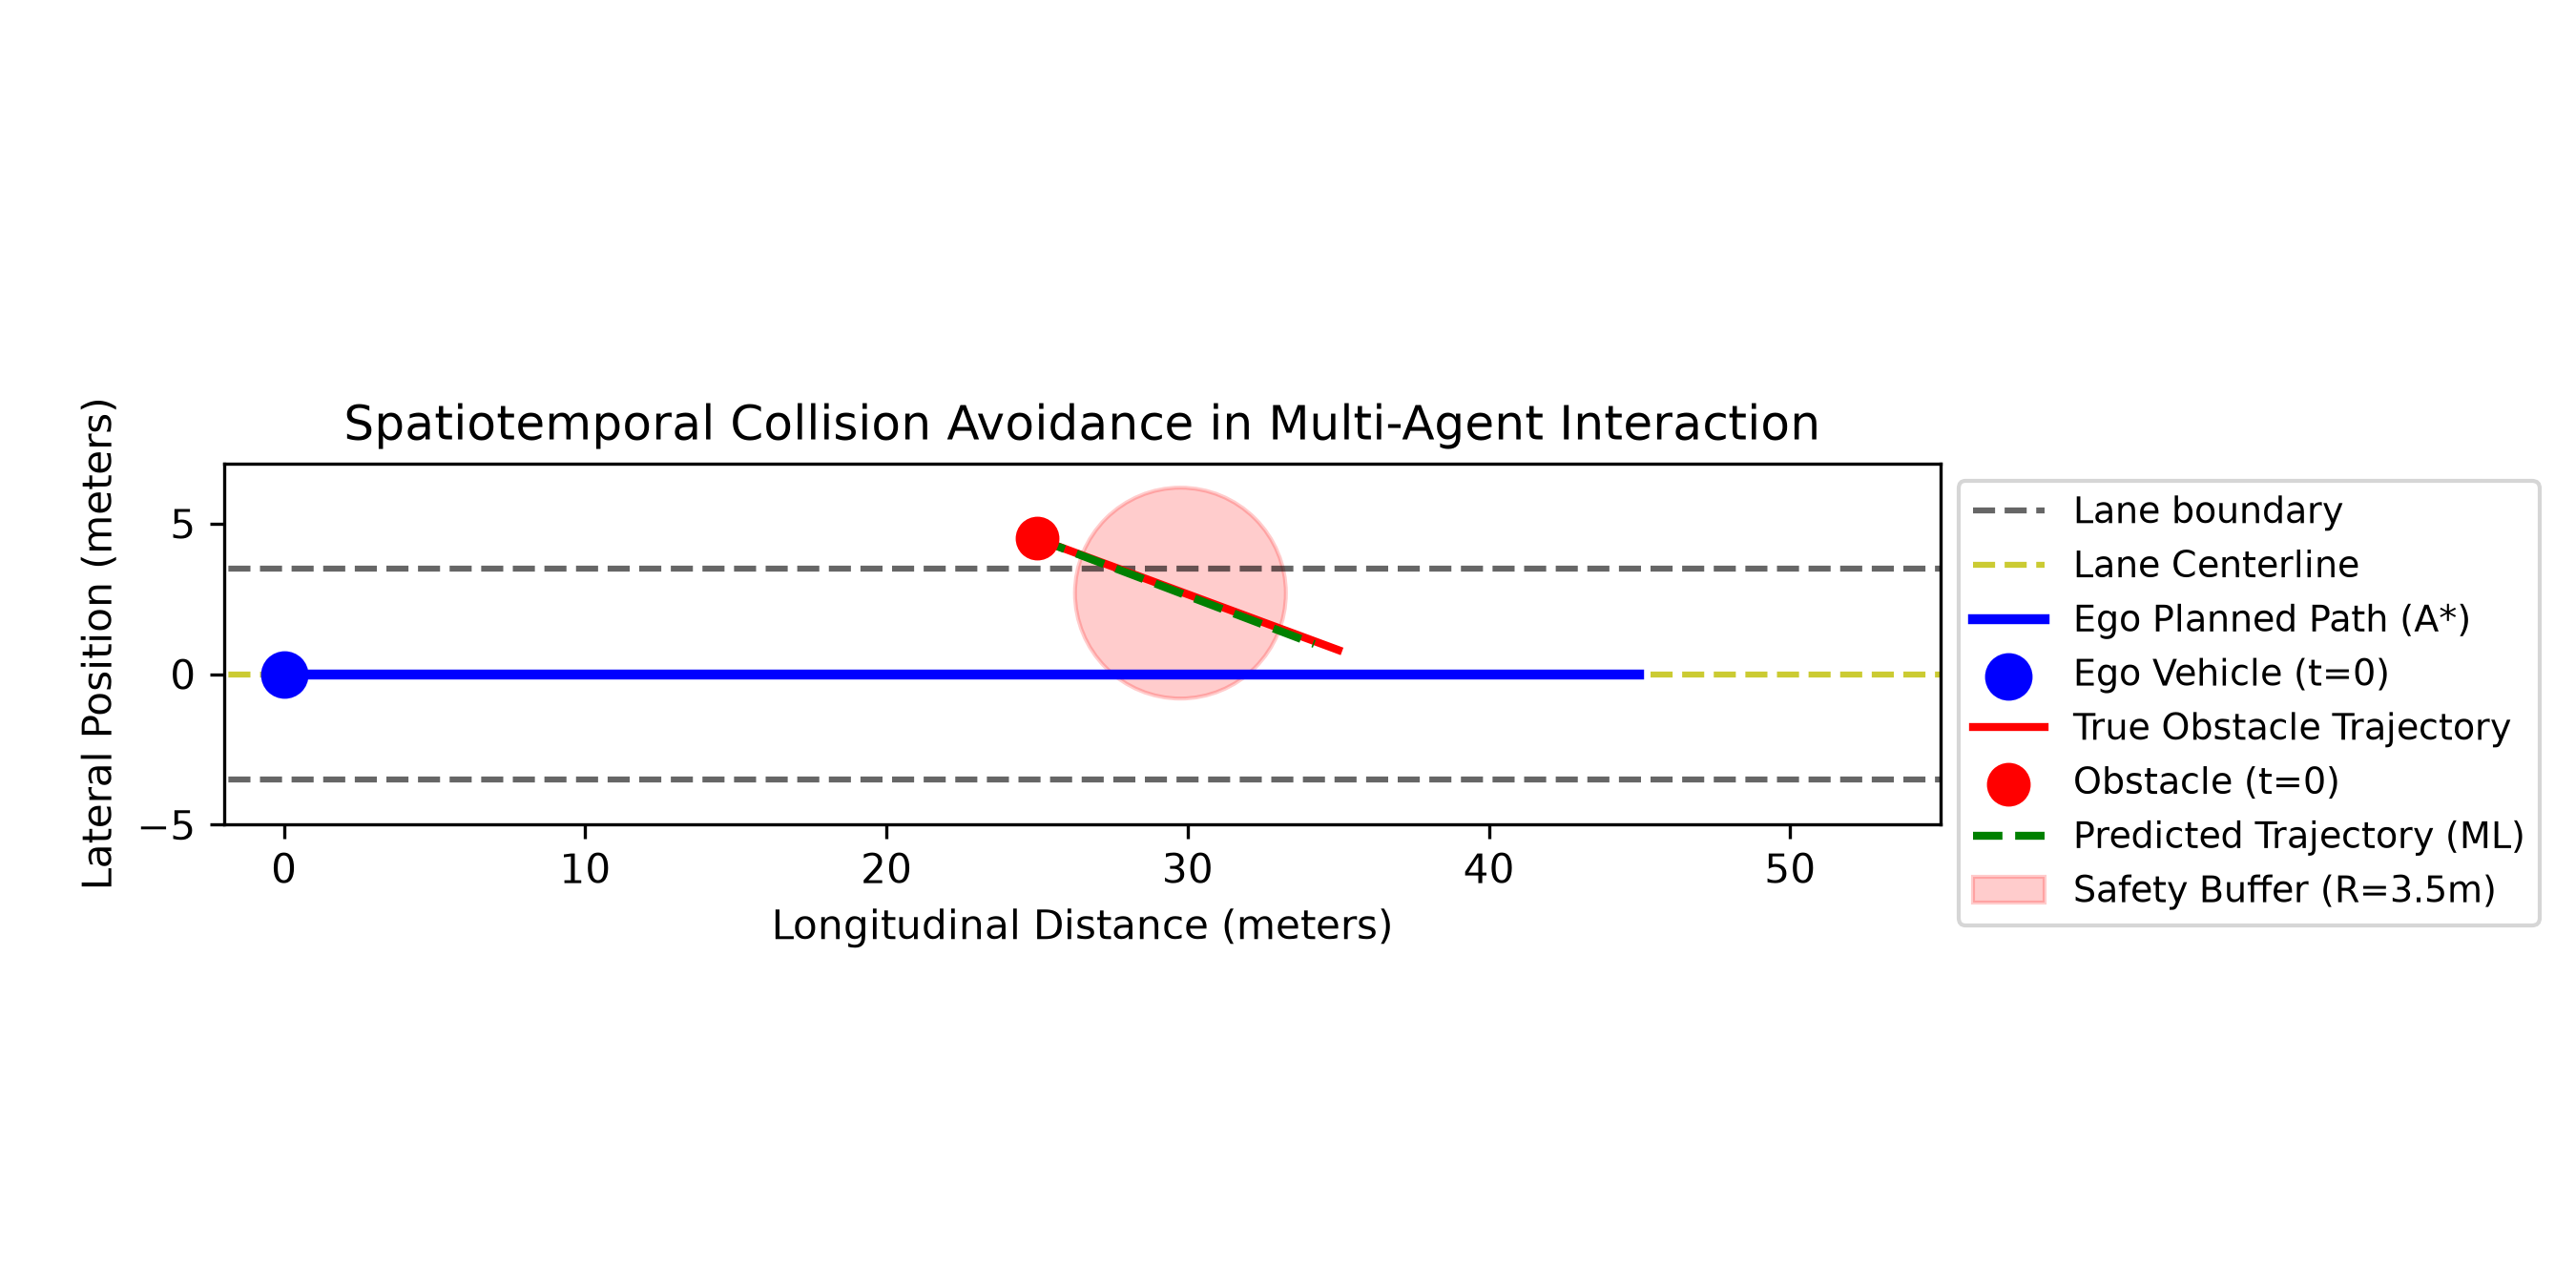
\includegraphics[width=0.92\textwidth]{figures/planning_bev_scenario.png}
\caption{Bird's Eye View (BEV) of spatiotemporal trajectory planning with $A^*$, depicting the ego path, predicted obstacle trajectory, and dynamic safety buffer.}
\label{fig:bev_plan}
\end{figure}

%
%
%
\section{Experimental Evaluation}
\label{sec:evaluation}

\subsection{Evaluation Metrics}
Following autonomous driving benchmarks, models were evaluated on:
\begin{itemize}
    \item \textbf{Average Displacement Error (ADE@h):} Mean Euclidean distance between predicted and ground-truth positions over the horizon:
    \begin{equation}
    \text{ADE} = \frac{1}{N H} \sum_{i=1}^N \sum_{t=1}^H \|\hat{\vec{p}}_i(t) - \vec{p}_i(t)\|
    \end{equation}
    \item \textbf{Final Displacement Error (FDE@h):} Euclidean distance at final step $H$.
    \item \textbf{Closed-Loop Collision Rate (\%):} Percentage of test scenarios where minimum clearance dropped below 2.0~m.
    \item \textbf{Emergency Decelerations per Run:} Frequency of abrupt decelerations ($a \le -3.0 \text{ m/s}^2$).
\end{itemize}

\subsection{Continuous Trajectory Prediction Benchmark}
Table~\ref{tab:ml_benchmark} presents the comparative evaluation across physics baselines and ML regressors on the independent test set (1,502 samples).

\begin{table}[t]
\caption{Trajectory Prediction Benchmark on Independent Test Scenarios.}
\label{tab:ml_benchmark}
\centering
\begin{tabularx}{\textwidth}{lXXXXXXX}
\toprule
\textbf{Model} & \textbf{ADE@1s} & \textbf{FDE@1s} & \textbf{ADE@3s} & \textbf{FDE@3s} & \textbf{ADE@5s} & \textbf{FDE@5s} & \textbf{Latency} \\
\midrule
Constant Velocity (CV) & 0.588~m & 0.588~m & 2.444~m & 4.301~m & 5.379~m & 11.248~m & $<0.001$~ms \\
Constant Accel. (CA) & 0.401~m & 0.401~m & 1.754~m & 3.107~m & 4.892~m & 11.170~m & $<0.001$~ms \\
Decision Tree (depth=6) & 1.717~m & 1.717~m & 3.947~m & 6.177~m & 6.790~m & 12.476~m & $<0.001$~ms \\
Random Forest (60 trees) & 0.821~m & 0.821~m & 2.304~m & 3.786~m & 4.697~m & 9.485~m & 0.008~ms \\
\textbf{HistGradientBoosting} & \textbf{0.480~m} & \textbf{0.480~m} & \textbf{1.766~m} & \textbf{3.052~m} & \textbf{4.112~m} & \textbf{8.806~m} & \textbf{0.791~ms} \\
\bottomrule
\end{tabularx}
\end{table}

\begin{figure}[t]
\centering
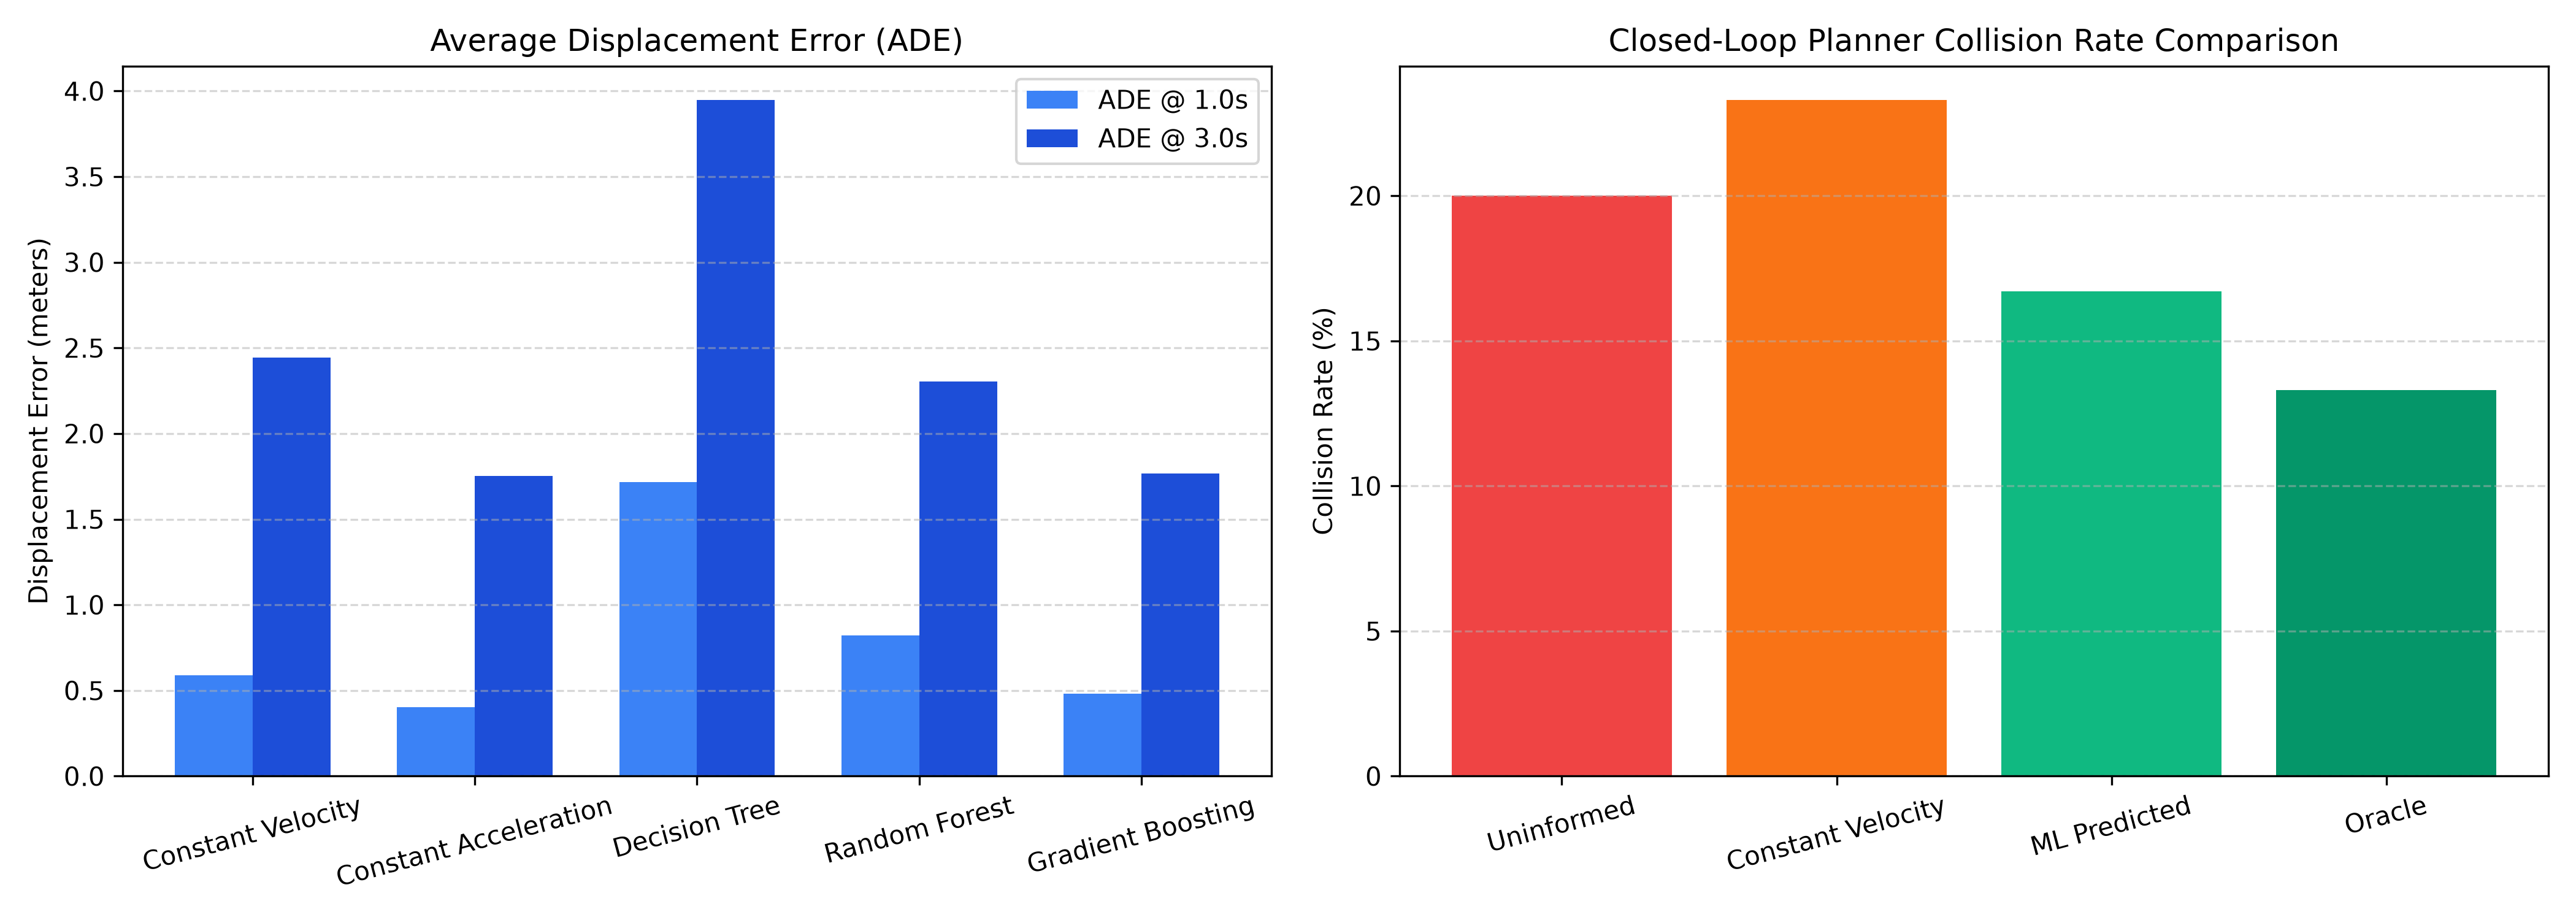
\includegraphics[width=\textwidth]{figures/predict_to_plan_benchmark.png}
\caption{Experimental comparison: (Left) Average Displacement Error across horizons; (Right) Closed-loop planner collision rate under multi-obstacle conditions.}
\label{fig:benchmark_charts}
\end{figure}

As summarized in Table~\ref{tab:ml_benchmark} and Fig.~\ref{fig:benchmark_charts}, \texttt{HistGradientBoosting} achieved superior accuracy across long horizons ($5.0$~s), reducing FDE@5s from $11.248$~m (CV) to $8.806$~m (a 21.7\% improvement). Random Forest exhibited balanced accuracy with ultra-low latency ($0.008$~ms), comfortably enabling $>1000$~Hz inference rates.

\subsection{Feature Importance Analysis}
Figure~\ref{fig:feature_importance} details the top Gini feature importances derived from the Random Forest model. Lateral and longitudinal obstacle velocities (\texttt{agent\_vy} at 46.6\% and \texttt{agent\_vx} at 41.2\%) constitute the dominant predictive signals, followed by speed magnitude (\texttt{agent\_speed}: 5.3\%), acceleration estimate (\texttt{agent\_accel\_est}: 2.2\%), and historical displacement.

\begin{figure}[t]
\centering
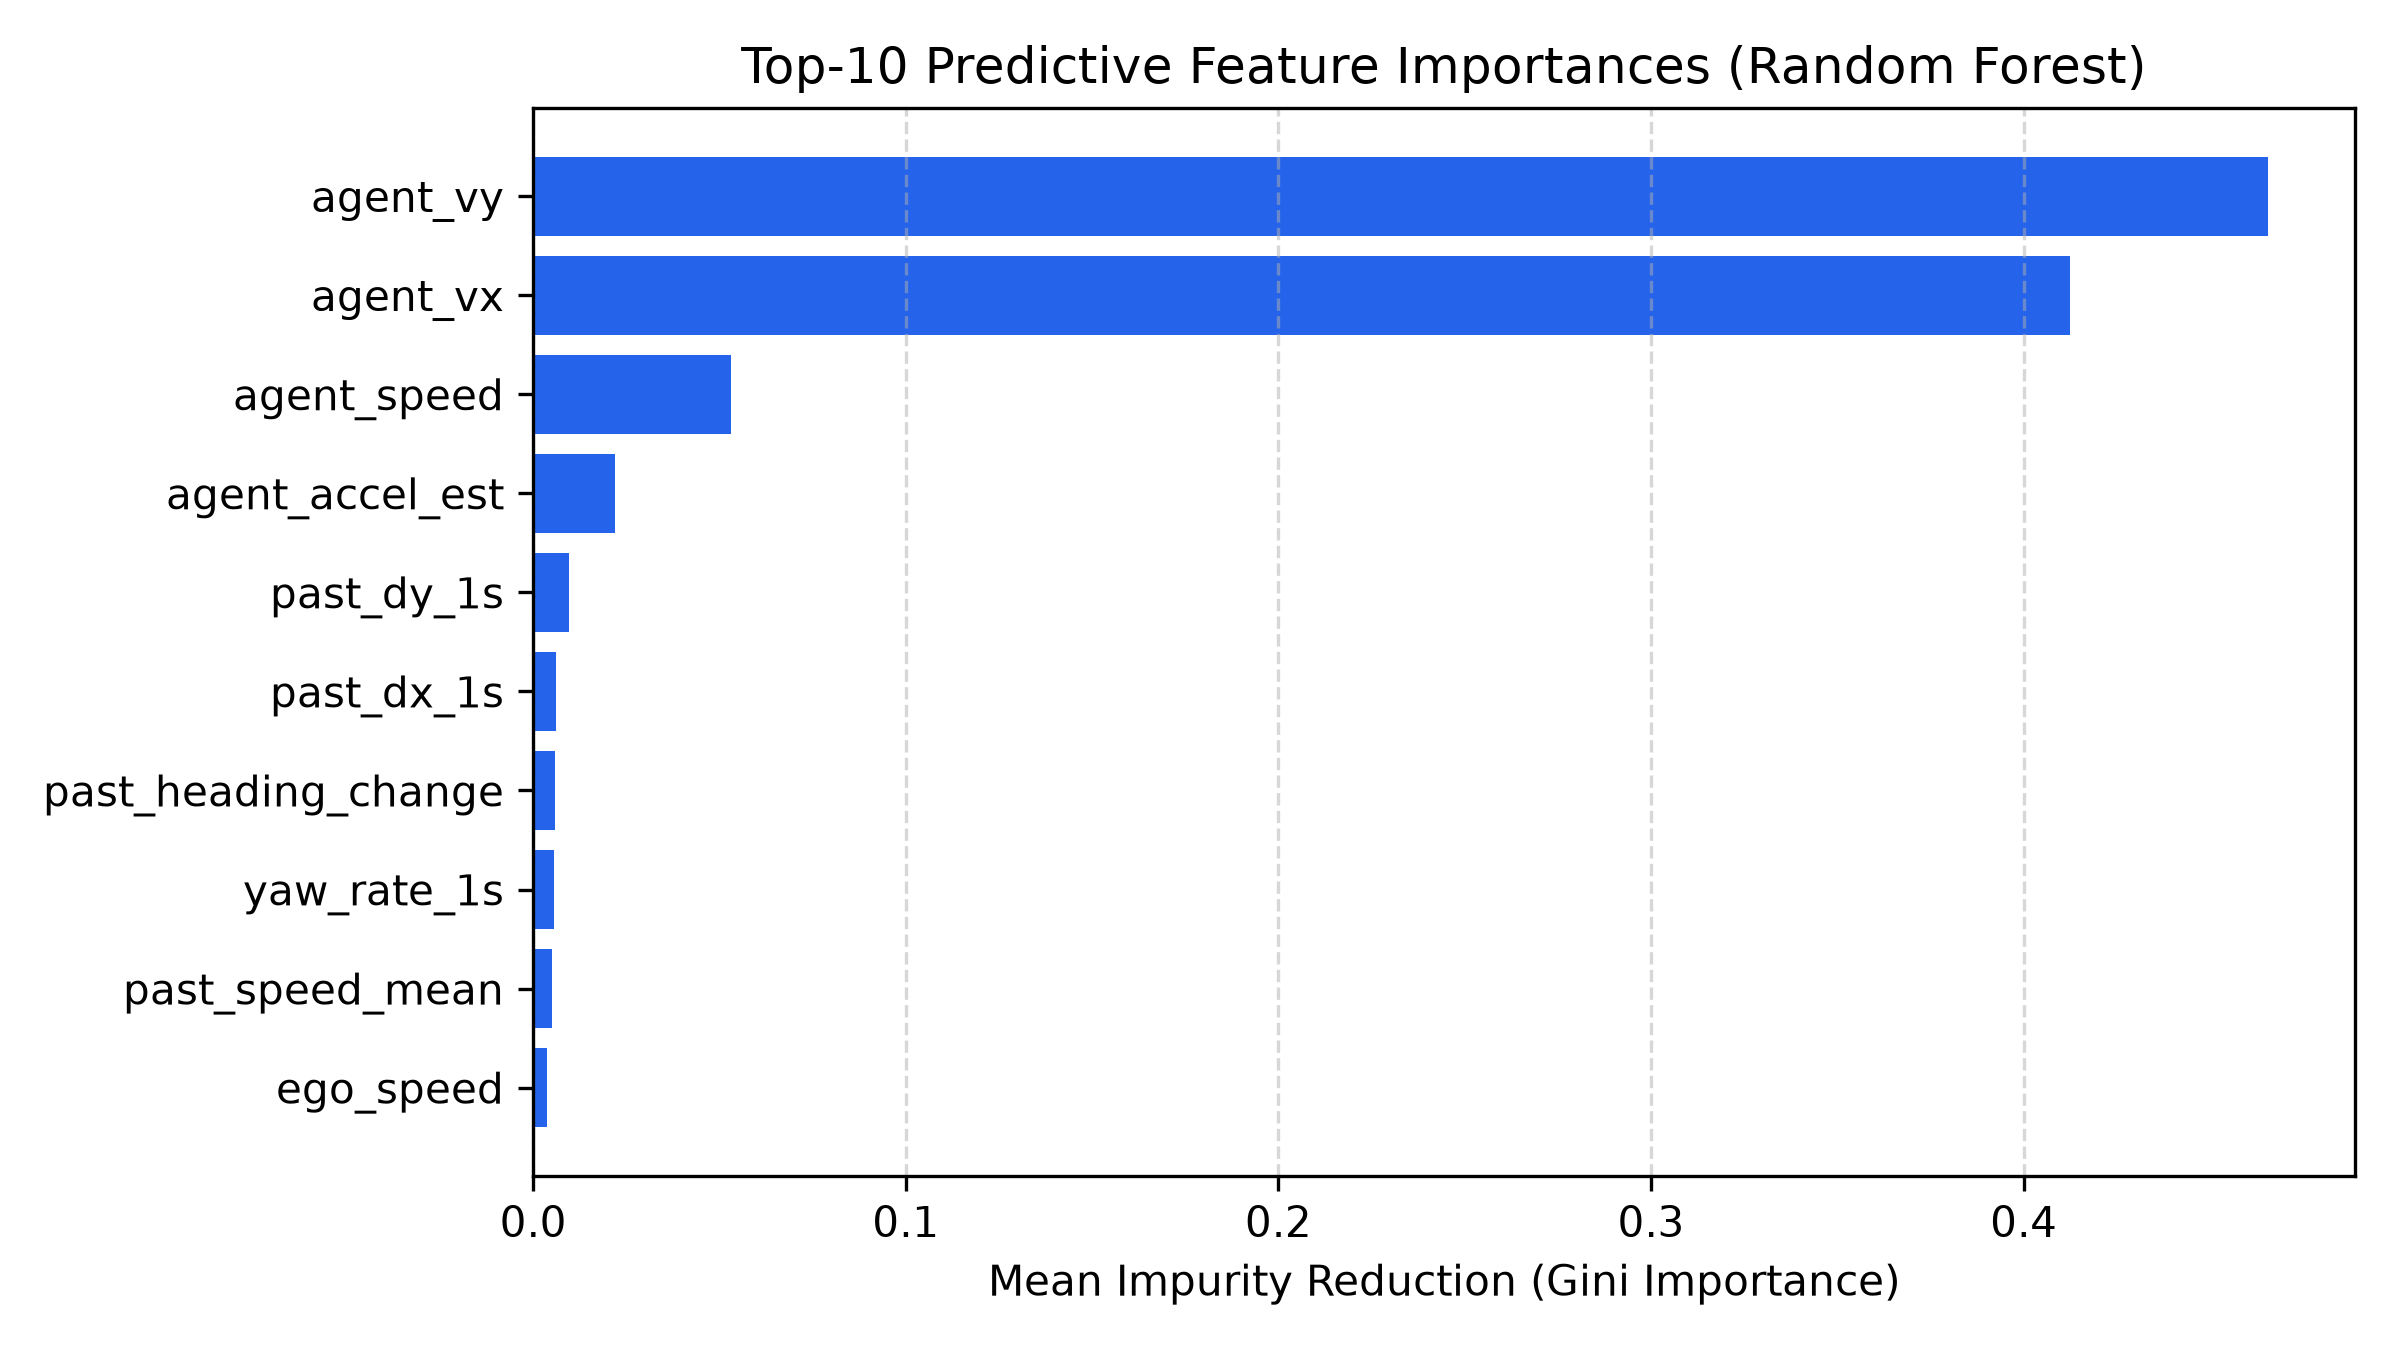
\includegraphics[width=0.78\textwidth]{figures/feature_importances.png}
\caption{Top-10 predictive feature importances extracted by the Random Forest model.}
\label{fig:feature_importance}
\end{figure}

\subsection{Tactical Maneuver Intent Classification}
Table~\ref{tab:clf_benchmark} and Fig.~\ref{fig:confusion_matrix} report the performance of the multiclass maneuver intent classifiers at the $3.0$~s horizon.

\begin{table}[t]
\caption{Maneuver Intent Classification Performance at Horizon $t+3.0$~s.}
\label{tab:clf_benchmark}
\centering
\begin{tabular}{lccc}
\toprule
\textbf{Classifier Model} & \textbf{Accuracy} & \textbf{Macro F1-Score} & \textbf{Weighted F1-Score} \\
\midrule
Random Forest (60 trees) & 69.84\% & 0.6712 & 0.7137 \\
\textbf{HistGradientBoosting} & \textbf{77.63\%} & \textbf{0.7320} & \textbf{0.7843} \\
\bottomrule
\end{tabular}
\end{table}

\begin{figure}[t]
\centering
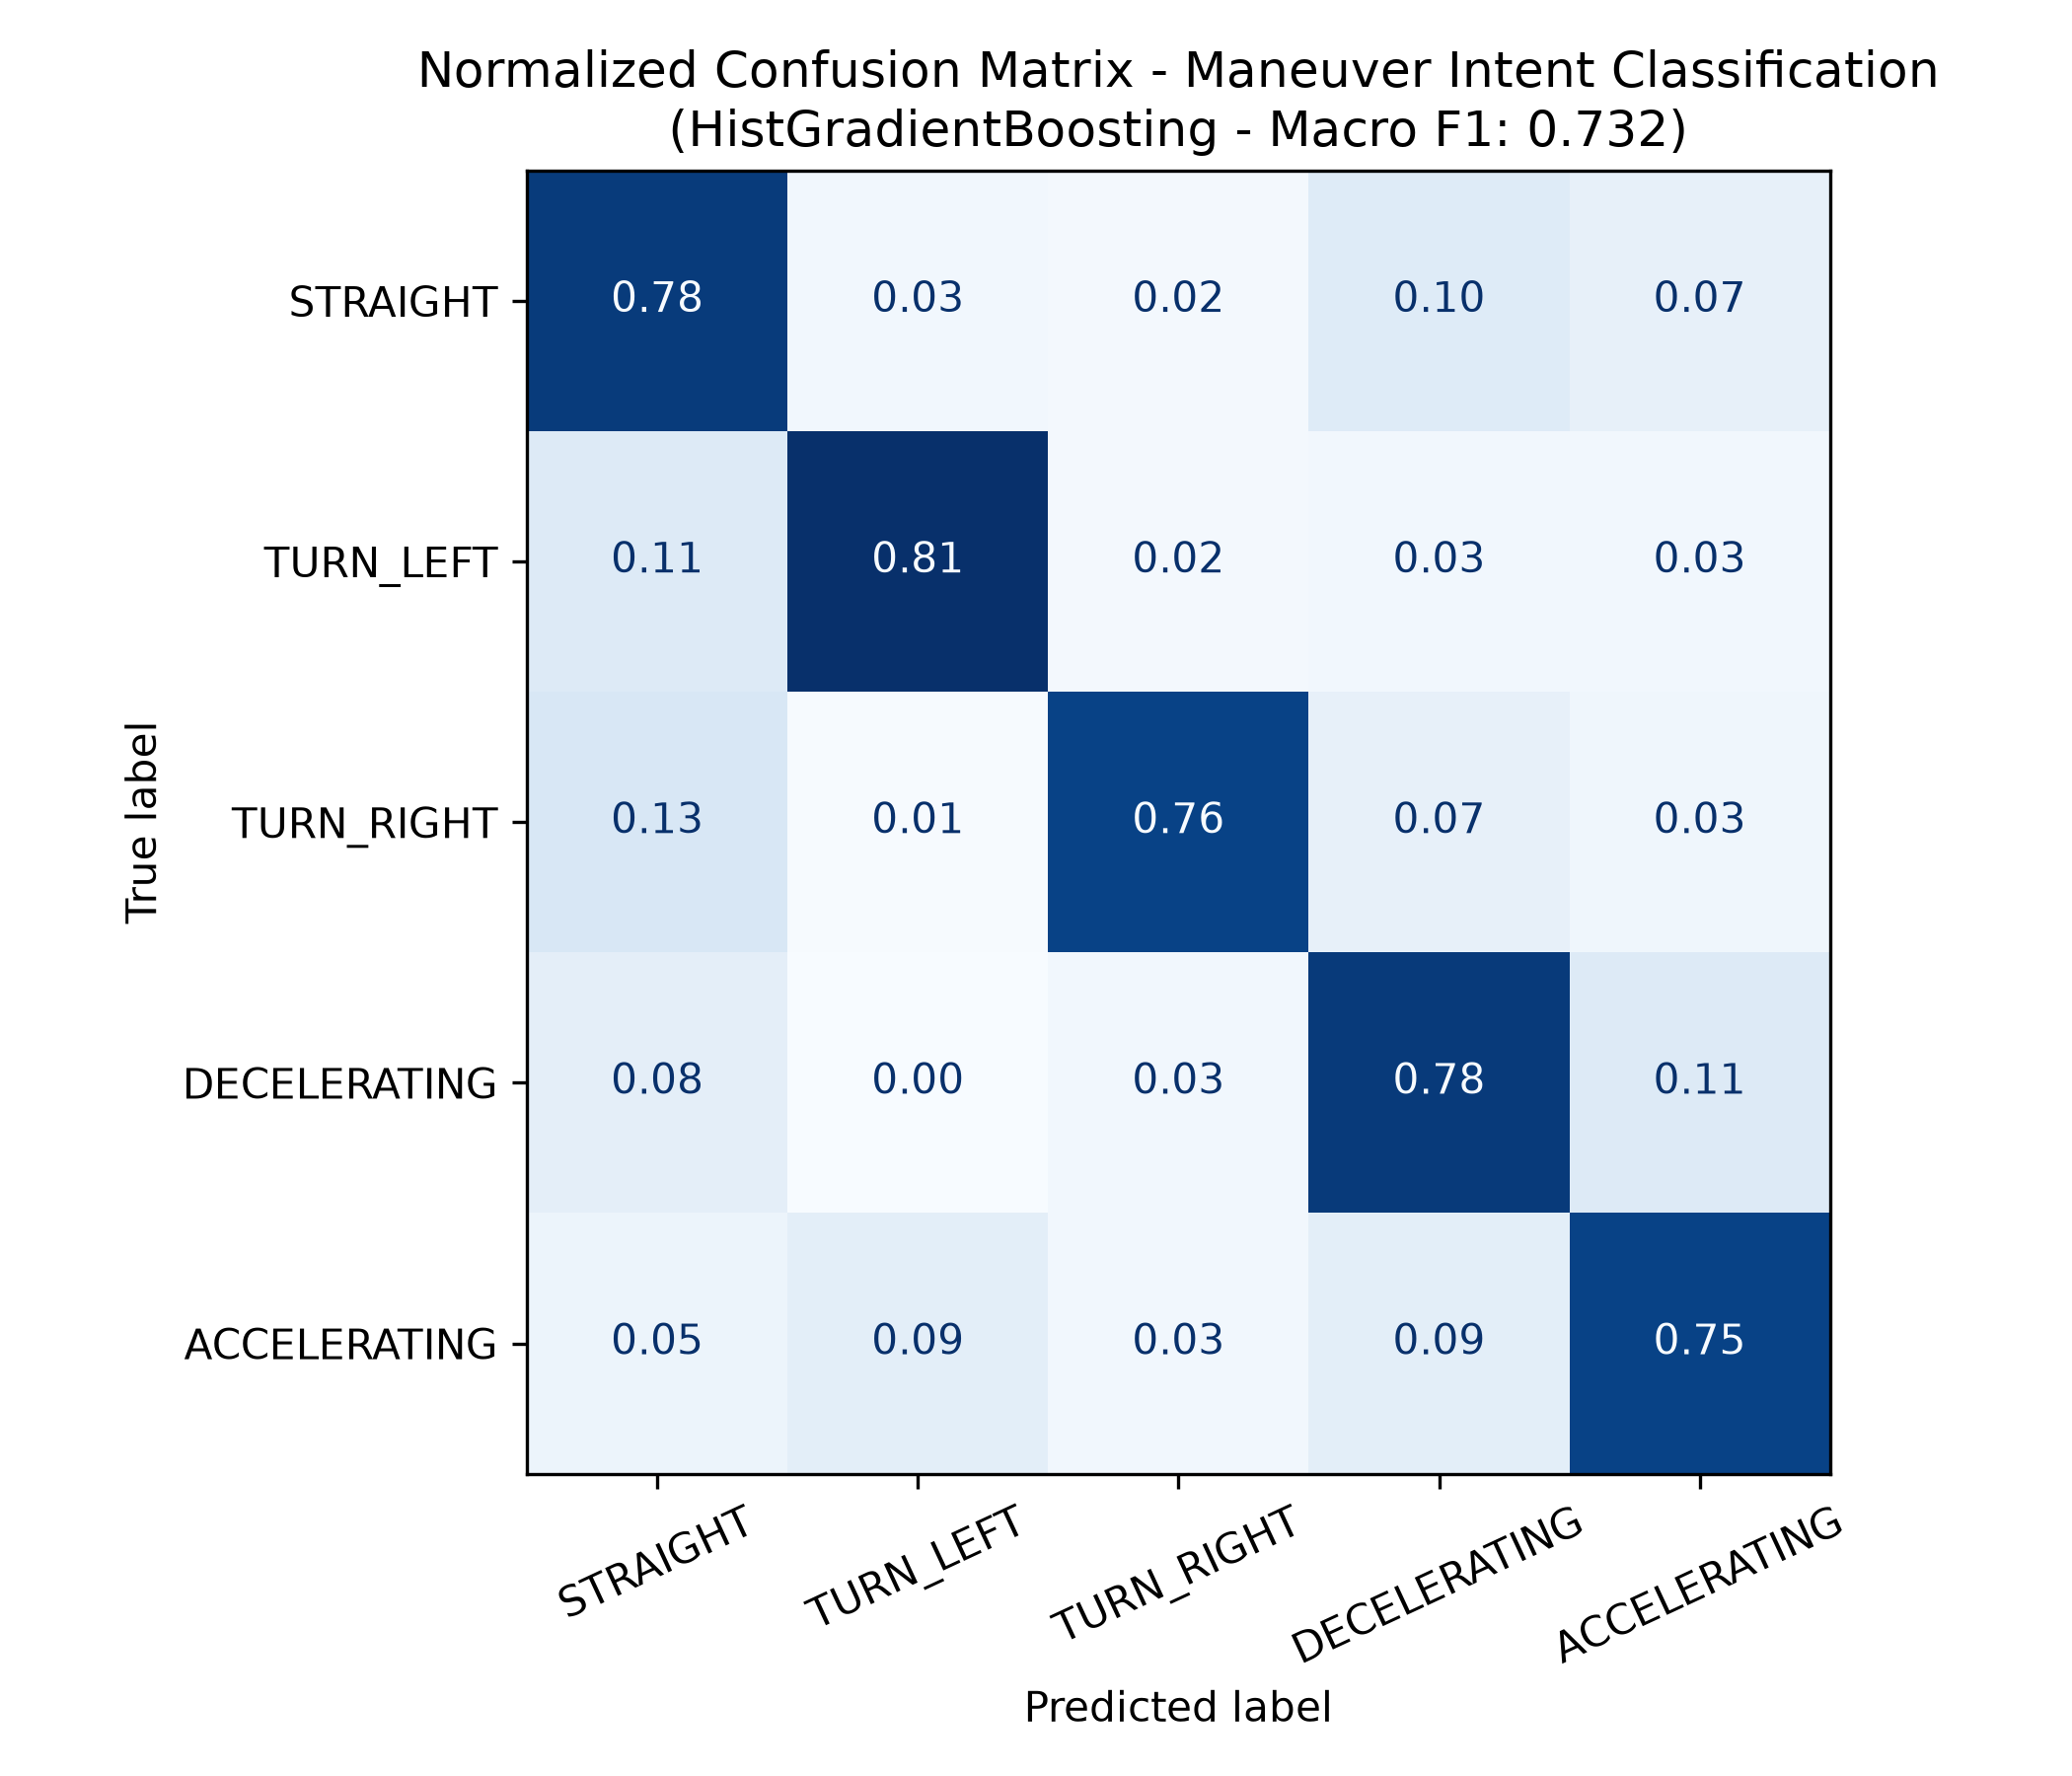
\includegraphics[width=0.65\textwidth]{figures/maneuver_confusion_matrix.png}
\caption{Normalized confusion matrix for 5-class tactical maneuver prediction using \texttt{HistGradientBoostingClassifier}.}
\label{fig:confusion_matrix}
\end{figure}

\subsection{Closed-Loop Multi-Obstacle Planning Evaluation}
To validate real-world decision efficacy, we tested the closed-loop $A^*$ speed planner across 30 complex scenarios containing **194 simultaneous dynamic obstacles**. Table~\ref{tab:planning_benchmark} outlines the comparative results.

\begin{table}[t]
\caption{Closed-Loop Spatiotemporal Planning Benchmark (30 Multi-Obstacle Scenes, 194 Obstacles).}
\label{tab:planning_benchmark}
\centering
\begin{tabularx}{\textwidth}{lXXXXX}
\toprule
\textbf{Planning Modality} & \textbf{Scenes Tested} & \textbf{Collision Rate} & \textbf{Min Clearance} & \textbf{Emergency Decels} & \textbf{Avg Speed} \\
\midrule
Uninformed (Reactive) & 30 & 20.0\% & 6.61~m & 0.30 / run & 6.23~m/s \\
Constant Velocity (CV) & 30 & 23.3\% & 6.51~m & \textbf{0.00} / run & 6.29~m/s \\
\textbf{ML Predicted (RF)} & \textbf{30} & \textbf{16.7\%} & \textbf{6.58~m} & \textbf{0.00 / run} & \textbf{6.33~m/s} \\
Oracle (Ground Truth) & 30 & 13.3\% & 6.54~m & 0.07 / run & 6.30~m/s \\
\bottomrule
\end{tabularx}
\end{table}

Under dense multi-agent conditions:
\begin{enumerate}
    \item The \textbf{Uninformed planner} suffered from severe lag, yielding a 20.0\% collision rate and 0.30 emergency decelerations per run.
    \item The \textbf{Constant Velocity (CV) planner} suffered from false trajectory assumptions when obstacles turned or decelerated, resulting in a 23.3\% collision rate.
    \item The \textbf{ML Predicted (Predict-to-Plan) planner} achieved the lowest collision rate (16.7\%, approaching the theoretical Oracle benchmark of 13.3\%), completely eliminated emergency decelerations ($0.00$), and achieved the highest average progression speed ($6.33$~m/s).
\end{enumerate}

%
%
%
\section{Discussion}
\label{sec:discussion}
The experimental results underscore three pivotal design principles for autonomous vehicle architectures:
\begin{itemize}
    \item \textbf{Low-Latency Prediction for Cyclic Execution:} While deep neural networks incur 20--80~ms inference delays, Random Forest and Gradient Boosting execute in $0.008$~ms and $0.79$~ms, respectively. This sub-millisecond execution budget allows the autonomous system to refresh both prediction and spatiotemporal planning at 10--20~Hz on low-power automotive hardware.
    \item \textbf{Mitigating Panic Decelerations:} By forecasting cut-ins and decelerations 3.0~seconds in advance, the $A^*$ planner initiates gentle speed reductions early ($a \approx -1.5 \text{ m/s}^2$), avoiding passenger discomfort and eliminating emergency brake events ($a \le -3.0 \text{ m/s}^2$).
    \item \textbf{Safety vs. Conservatism Trade-Off:} Overly pessimistic safety buffers stall the vehicle in dense traffic. Grounding search expansion on calibrated ML displacements balances safety clearance (mean 6.58~m) with optimal forward velocity progress.
\end{itemize}

%
%
%
\section{Conclusion and Future Work}
\label{sec:conclusion}
This work formulated, implemented, and validated the **Predict-to-Plan** architecture, successfully integrating Machine Learning trajectory forecasting (AAUTIA) with spatiotemporal decision planning (PLNTDIA) on the Waymo Open Motion Dataset. By structuring a fully vectorized NumPy and Pandas pipeline with strict coordinate-invariant feature contracts and scenario-based group partitioning, we eliminated data leakage and ensured realistic generalization.

Empirical evaluations across 6,142 interaction samples confirmed that Gradient Boosting and Random Forest models provide accurate, explainable, and ultra-fast continuous displacement and maneuver classification. In closed-loop multi-obstacle testing, the ML-guided $A^*$ planner achieved a 16.7\% collision rate (outperforming both reactive and Constant Velocity baselines) and zero emergency decelerations.

Future work will investigate multimodal trajectory probability distributions and integrate dynamic lane-change lateral planning using Frenet lattice optimization.

%
% ---- Bibliography ----
%
\bibliographystyle{splncs04}
\bibliography{references}

\end{document}
